
\chapter{Approach}\label{chapter:realization}

In this chapter, the main approach of this thesis is presented. The chapter starts with an abstract description of the approach with the aim of providing a high-level overview of the underlying concepts. Then, a list of requirements and desirable quality attributes is given on the basis of which the approach is later evaluated. The section that follows gives a concrete example of how the system may be realized. For this, an exemplary technology stack is presented, whereby each of the employed technologies is discussed in detail. This part builds the basis for the subsequent chapter, where a system based on the presented technologies is evaluated.

%
%
%
%
%
%
%
%
%
%

\section{Concept}

\todo{einstieg ueberarbeiten}The approach follows a service-oriented architectural paradigm whereby the system is composed of a number of \emph{services}. Each service provides an offering to other services. Such offering may be some kind of data or functionality. All services of the system are working together in synergy to achieve a common goal. 

Services expose their functionality by means of topics in a publish-subscribe environment. The method of exposition is data-centric: instead of providing \emph{methods} that other services may invoke (RPC style), services offer \emph{data}. Any service interested in receiving a certain kind of data listens in on a topic on which such data is published. This approach greatly helps to decouple the system as services have no reference to one another. As a result, services may evolve without having to deal with interface interdependencies. Promotes decoupling
Although this makes request-response-style communication rather difficult (as it is discouraged) it is still possible. 

A major goal of the approach is scalability, and in particular, horizontal scalability. Therefore, replication is key. The service-oriented approach alleviates this tremendously, provided that certain design principles are applied. Hence, throughout the design and implementation of the envisioned system, several design goals need to be kept in mind. Firstly, services ought to be \textbf{stateless}. Statelessness facilitates replication as sharing state among many instances proves to be difficult. Consistency is hard to achieve and locking mechanisms may become a bottleneck.\todo{more on consistency models this in tanenbaum...} Furthermore, services should be \textbf{fine-grained}. A high-resolution granularity allows for detailed control over which services should be replicated. That way, computational bottlenecks can be more easily singled-out and eliminated. An added benefit is increased extensibility and faster software updates. However, trade-offs need to be considered. If services are too fine-grained, they need to communicate more, and as a result, the communication channel might become a bottleneck. Furthermore, too many services unnecessarily increase complexity.

Another design goal to keep in mind is \textbf{isolation}. Services should have limited knowledge of both, location and topology. The aim should be to hide anything that isn't directly related to the reception of data. Through that, loose coupling is achieved. One aspect of isolation is self-containment. Services should be kept together with all their dependencies as a single unit that may be deployed on any hardware platform. By packaging services in self-contained environments, they may be moved between different computing nodes. This property is the most important one to achieve cloud scalability. Commonly used tools to facilitate this are virtualization and containerization.

The last question that remains is how services are connected. Since services may be duplicated and migrated between computing nodes, special emphasis needs to be put on location/relocation transparency and dynamic topology management. In the approach, the use of virtual overlay networks is suggested for this purpose. Especially challenging is the fact that the overlay must work on top of a substrate network made up of numerous globally dispersed nodes, of which some continuously change their location. As a result, the substrate network is exceptionally unreliable.

\paragraph{}

\begin{figure}[htpb]
  \centering
  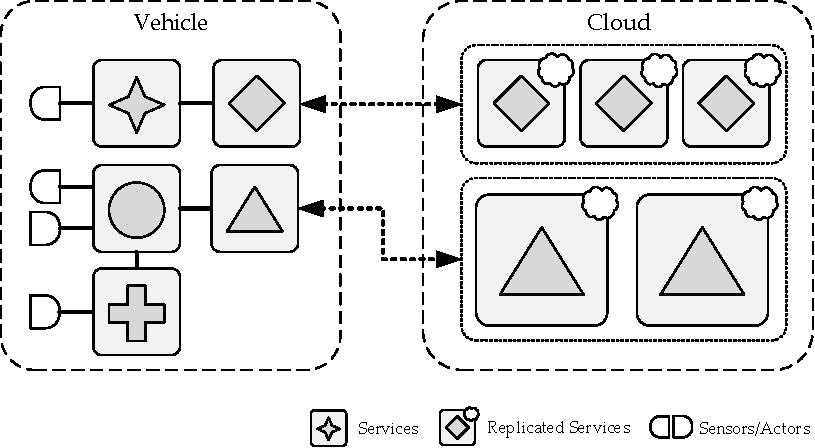
\includegraphics[width=0.8\textwidth]{figures/idea.pdf}
  \caption[Conceptual sketch of the approach]{Conceptual sketch of the approach, demonstrating location transparent replication of services in the cloud}\label{fig:idea} 
\end{figure}

\autoref{fig:idea} presents a schematic view of the approach. The box on the left-hand side represents a vehicle. In the vehicle, several interconnected services are deployed. What is not depicted, but naturally given, is that these services run on distributed embedded devices spread over the vehicle's E/E system. On the right-hand side, the cloud is depicted, which, in actuality, is a collection of high-performance computing nodes. Vehicle and cloud are physically separated and connected via some sort of network, which is accessible, \eg , by means of 5G. As can be observed in the figure, some of the vehicle-intrinsic services are replicated in the cloud (\ding{117}, \ding{115}). Examples of such services could be functions for predicting trajectories, gaze detection, or machine learning algorithms. The duplication and varying size of the service boxes depicted in the image is indicative of horizontal and vertical scaling, respectively. It doesn't always make sense to replicate services in the cloud, \eg , because they are computationally inexpensive, or because they require access to sensors and actors which can only be found in the vehicle (\ding{70}, \ding{108}, \ding{58}). Those services have their firm place within the vehicle and are referred to as \emph{fixed} services. Their counterpart, \ie , services that may migrate to the cloud are called \emph{volatile} services. The discrepancy between fixed and volatile services emphasizes the need to split functionality into fine-grained services so that computational bottlenecks can be isolated and then eliminated. A good advice is to extract services connected to sensors and actors in minimal services ("\emph{access services}") that do nothing but provide a low-level interface to sensor data.

\paragraph{Key Challenges}

In this section, an approach was presented to offload computations to the cloud. To achieve this, the approach suggests to split functionality into fine-grained services that may be replicated and migrated smoothly between vehicle and cloud. The problem at hand can be categorized in three key challenges which need to be addressed:

\begin{enumerate}
\item \textbf{Reliable Information Exchange}: Services must be able to communicate in a reliable manner, without needing direct references to one another.
\item \textbf{Isolation}: Services need to be packed in self-contained execution environments with all their dependencies.
\item \textbf{Connectivity}: Services need to be able to autonomously create connections between each other and stay connected, regardless of where they are.
\end{enumerate}

%
%
%
%
%
%
%
%
%
%

\section{Requirements and Quality Attributes}
The previous section already touched on desirable quality attributes to keep in mind when implementing the approach. Still, a rigor requirement analysis is needed in order to be able to thoroughly evaluate it. To this end, a detailed requirement list is presented which an implementation of the envisioned system should aim to fulfill. The list is loosely based on the work of \citeauthor*{o2007quality} \cite{o2007quality}.

\todo[inline]{More info: Dependable systems [Kopetz, Verissimo]: Availability, Reliability, Safety, Maintainability}

\paragraph{Availability.}
Availability states how likely it is that, at any given point in time, a system is ready to be used by its users \cite{tanenbaum2017distributed}. The period in which a system or service is unavailable is called \emph{downtime}. Sources of downtime can be, \eg , maintenance work, temporary congestion, or any kind of failure. A design goal when building and running software systems is to minimize downtime, and thereby maximize availability. This goal is not trivial to achieve as many sources of decreased availability are hard to predict, \eg\ in case of hardware failures. A key technique for handling downtime is redundancy, whereby critical systems, or those susceptible to downtime, have a replacement ready to be used at all times. A prerequisite for redundancy to take effect is that the system features quick failure detection and smooth transition mechanisms so that it can quickly reroute requests to the redundant service.

\paragraph{Reliability.}
Reliability states how long a system can continuously run without failure. A reliable system is available for prolonged periods of time without interruption. Although reliability is related to availability, there is a clear distinction between the two. While reliability states a continuous period of operability, availability concerns operability at a given point in time. For example, a system that works fine most of the time but becomes unavailable for a few milliseconds every hour is highly available, but not reliable. Hence, a highly reliable system is not necessarily a highly available one and vice versa \cite{tanenbaum2017distributed}.

In real-time systems, even a temporary failure could have disastrous effects. If the system is a hard real-time system, a single missed deadline is even equivalent to a complete system failure. Ensuring reliability is therefore of utmost importance. As with availability, a way to mitigate the effects of poor reliability is redundancy.

Special precautions need to be taken for \emph{distributed} systems as their communication channels are inherently unreliable \cite{tanenbaum2017distributed}. In practice, this means that the messaging system needs to provide guarantees for a timely and robust message delivery. In addition, certain assurances must be given, \eg , that messages are delivered in order or that every message is delivered only once \cite{o2007quality}. 

\paragraph{Safety.}
The safety of system states how resilient \wrt\ failures it is, and in case a failure occurs, how well it can handle it. A safe system manages to protect the health and wellbeing of humans involved in the operation of the system and its surrounding bystanders.
As human lives are at stake in road traffic environments, vehicles are a prime example of systems that need to be safe.

Critical functions need to operate in a fail-operational fashion, \ie , in case they fail, the situation needs to be handled gracefully, without putting the passengers in danger. To this end, special precautions need to be taken throughout the whole process of development, provisioning, operation, and service of functions. ISO 26262 \cite{iso201126262} provides the standards that vehicular E/E systems need to adhere to in order to fulfill the necessary safety requirements. Different parts of the system need to be compliant to different classes of safety, indicated by automotive safety integrity levels (ASILs).

\paragraph{Interoperability.} 
In systems composed of a number of heterogeneous components that interact with each other, there needs to be a common set of rules and semantics that all involved parties must comply with. If such rules exist, so that diverse components may interact with each other, they are said to be interoperable.
A major barrier to interoperability is vendor lock-in, or more general, platform lock-in. Lock-in describes a situation in which a technology is rooted so deep within the system that it can barely be removed without considerable effort. Lock-in is detrimental to system design as it creates dependencies, and thus, enforces tight coupling. A way to achieve a high degree of interoperability is to avoid proprietary, closed-source solutions and to favor open standards instead.


\paragraph{Security.}
In road traffic, flaws in a system's IT security have direct implications for safety. Since safety is of utmost importance the same is true for security. 

Several developments call for an increased emphasis on security.

Increasing amounts of code in vehicles -> increased attack surface

increased connectivity -> exposed to the public 

autonomous driving: software-controlled actuator systems. -> malicious attackers might remote control vehicle


Precautions:

Proper isolation of software components is needed.

state-of-the-art encryption and security measures are needed to ensure the integrity, authenticity, and confidentiality of the system.

Data in the cloud needs to be stored safely.


\paragraph{Performance.}
Services in an automotive SOA are deployed on embedded computing devices that must fulfill real-time requirements. This is in stark contrast to services in traditional SOAs that often run on high performance machines. The resource constrained nature of embedded systems requires special operating systems, communication technologies and programming techniques.

low response times, high throughput and timeliness (Real-time requirements must be fulfilled)

performance is influenced by scalability: scalability can help to increase performance

Measures:

Low network overhead must be given

support for compiled programming languages must be given

no unnecessary overhead may be incurred


\paragraph{Extensibility.} 


It must be easily feasible to extend an SOA with new services and to update existing ones. The provisioning of new functionality must be possible not only at design-time but also at run-time. Modern automotive software architectures must deal with the fact that vehicular functions may be modified, added, or unlocked at run-time through automatic software updates.

\paragraph{Adaptability.}
Services deployed in a moving vehicle are exposed to a rapidly changing environment. Systems may unexpectedly fail, e. g. due to external forces. Automotive E/E architectures must be able to quickly react to such circumstances. Furthermore, services should be portable to facilitate repartitioning. For this reason they must adapt to run on different hardware platforms.

\paragraph{Testability.}
There are many ways in which a distributed system may break. Since operational safety is of paramount importance in automotive, testability is a key requirement. Components of an SOA must be testable in isolation as well as in interplay with other components. For this purpose, modern software development employs continuous integration tools that help to continually validate the correctness of a system throughout the whole development cycle. Automotive E/E architectures need to be adapted to make it feasible to employ such development practices.


\paragraph{Scalability.}
Scalability is a system's ability to handle increased computational demand by means of expansion. Generally, a distinction between two types of scalability is made: horizontal scalability, by which workload is distributed across an increased number of nodes (scaling out), and vertical scalability, by which a single node is upgraded with more powerful hardware (scaling up) \cite{tanenbaum2017distributed}. While vertical scalability is easier to realize, horizontal scalability scales much farther. This is, because at a certain point, it becomes cheaper to add entire nodes, than to further upgrade a node with increasingly expensive hardware.

A technique to achieve horizontal scalability is to replicate individual components and to deploy them on physically separated hosts to bypass computational and networking bottlenecks. Under certain circumstances it might be advisable to deploy such replications, or even the whole system, in the cloud, in order to offload computations. Cloud infrastructures often have means to dynamically scale out in an elastic fashion, depending on demand. This has the added benefit that also administration effort is offloaded, which may reduce operational expenses \cite{vaquero2011dynamically}.

Similarly, the messaging system must allow for the easy addition of components without negatively affecting performance.


\section{Realization}


\subsection{DDS as Messaging Middleware}

DDS is a promising candidate for a middleware that fulfills requirements to a satisfying degree.


Why DDS?

\paragraph{Dynamic Service Discovery.}

\paragraph{Data Centricity.}

\paragraph{Asynchronous Messaging.}

\paragraph{Location Transparency.}

\paragraph{Decentralization.}

\paragraph{Platform Independence.}


\subsubsection{Failover Mechanism}

DDS has ways to ensure reliable communication, even over unreliable transmission channels. For example, it allows for the realization of a failover mechanism which allows a failed service to be replaced by a backup service in a smooth and performant fashion. 

When DDS "observes" that a given service is unresponsive it automatically instructs another service to take over, provided that one exists. This mechanism is realized via the QoS policies \ownership , \ostrength\ and \liveliness\ . 

By assigning a topic the \ownership\ value "\qos{exclusive}" one can specify that only a single data writer may write to that topic at any given time. Which data writer is given that prerogative is determined by the data writer's \ostrength\ value. The data writer that possesses the higher value is eligible to write to the topic.

\liveliness\ is used to determine whether a data writer or data reader is "alive", \ie , responsive. For data writers, it is sufficient that it writes within a specified time interval in order to be considered "alive". For data readers, on the other hand, there are several ways in which it can signal liveliness. One way is to send continuous "heartbeat" messages.

\ownership\ can be combined with \liveliness\ to realize a failover mechanism.
\todo[inline]{how exactly?}


\subsubsection{DDS for Automotive Systems}

Automotive software systems have previously relied -- and, to some degree, will continue to do so -- on low-level, low-bandwidth transport protocols such as CAN, LIN, etc. For the longest time, networks stacks based on those protocols were sufficient to meet the basic requirements of delivering vehicular sensor data and x-by-wire functions. However, driven by the emergence of innovative functions, the demands for vehicle intrinsic networks are skyrocketing. In particular, more and more sensor data from increasingly bandwidth-hungry sensors, such as cameras and LIDARs is feeding into advanced systems such as ADAS. At the same time, these functions require computational capabilities that go way beyond of what is possible with the microcontrollers typically used in traditional ECUs. High-performance computer systems based on high-level operating systems, supported by bandwidth-friendly networking protocols are needed to meet the new requirements. A new generation of low-level network protocols found their way into the vehicle. Notable mentions are FlexRay, and TSN. A question that remains is whether DDS is a suitable choice for the use within vehicles, and whether DDS may be used efficiently on top of these lower level protocols. \citeauthor*{bouhouch2013dds} have shown \cite{bouhouch2013dds} that DDS is indeed a suitable middleware to be used in vehicular networks.


DDS is designed for resource constrained real-time applications such as sensor networks or industrial automation.

DDS allows to configure how much of a system's resources an DDS-enabled application may use. Consequently, it is the middleware's responsibility to allocate resources as needed while still staying within the specified boundaries. At the same time, priorities aligning with the application's QoS settings need to be considered. DDS takes this burden off the programmer's shoulders.



\subsubsection{Separation of User Data}

The presented approach relies on a single cloud infrastructure, while at the same time, a vast number of customers need to be served. This poses a challenge concerning the separation of data. Confidentiality and privacy of user-specific application data must be preserved. Similarly, the result of a computation commissioned by a specific vehicle must be returned to exactly that vehicle, and no one else. 

Gladly, DDS offers a solution to this. In DDS, topics are not restricted to a single domain, \ie , they may be reused in multiple domains. If, \eg , a publisher belongs to \texttt{Domain $\alpha$} and publishes data on \texttt{Topic A}. Then, a data reader that reads from \texttt{Topic A} but belongs to \texttt{Domain $\beta$} may not read the data. Therefore, through domains, the same application may be reused several times, while keeping topic data separate. This principle is take advantage of in the presented approach: Domains are used to separate user data, such that for each user there is one user-specific domain.




\subsection{\docker\ as Containerization Technology}

\docker\ is a promising technology for pr

\paragraph{Innovation Pressure}(not docker specific) calls for fast development cycles -> CI/CD

\paragraph{Portability} Containers need to run in vehicles and cloud -> \docker is available on many platforms, ARM version is fully functional

\paragraph{Light-weight}: Important for embedded systems, provides: fast spin-up, low overhead

\paragraph{Flexible network interfaces}: provide connection between distributed containers


\subsubsection{Multi Platform Compatibility} 
The primary purpose of containerization is to build portable execution environments that may run on a broad range of computing systems. Generally speaking, portability of containers is restricted to software compatibility, \ie , containers may run on a variety of different operating systems. However, since containerized applications run directly on the kernel of the host system -- and do not employ virtualization -- they are not portable between different hardware architectures. \Ie , applications packed in containers are not binary compatible. For instance, given an application that was built to run on a x86-based processor and packaged in a container. The same container will not run on a different processor, \eg\ one which is ARM-based. This poses a challenge for the approach at hand. Embedded systems are often based on particular hardware architectures which are tailored towards operation in resource constrained environments. Computing nodes in a data centers, on the other hand, are typically based on architectures aimed at providing a maximum level of performance, such as x86. Given that the envisioned scenario exactly matches this use case, this problem is of particular interested for this thesis.

Several approaches exist to tackle this problem. QEMU... This approach turned out to be unsuitable for the intended use case as multicast is not well supported by QEMU.


\subsubsection{Containerized Services}
Method: pack each service into a separate container.


\begin{figure}[htpb]
  \centering
  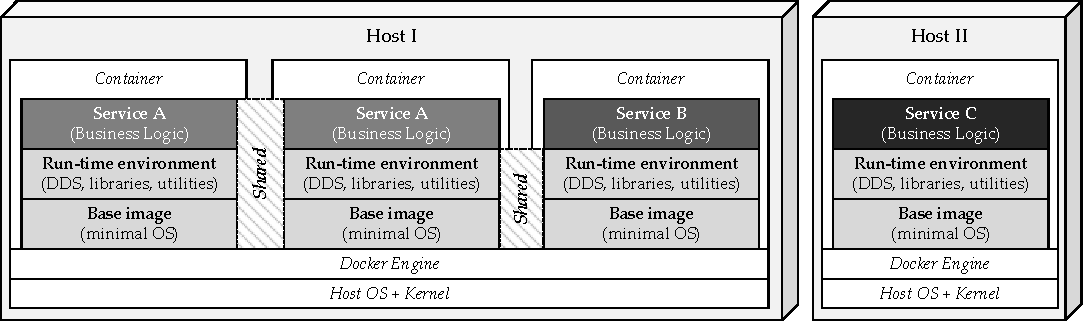
\includegraphics[width=\textwidth]{figures/docker-sharing}
  \caption[An example of containerized services]{An example of four containerized service instances, some sharing common logic to save disk space and facilitate fast updates}\label{fig:images} 
\end{figure}



\section{Container Networking with \wnet}
\wnet\ is an open source project\footnote{\url{www.github.com/weaveworks/weave}} which is developed by a global team, mostly employed by the London-based software company \emph{Weaveworks}\footnote{\url{www.weave.works}}. The purpose of \wnet\ is to provide advanced overlay networking capabilities for \docker\ containers. As such, is designed to make up for the shortcomings of \docker 's built-in overlay networks, and more specifically, their lack of encryption and multicast support. By means of \weave\ overlay networks, dispersed containers deployed on physically isolated hosts around the world, may communicate as if they were connected via LAN. From a containerized applications' viewpoint, it does not matter whether its peers are located on the same host or within a data center on the other side of the world. 

\paragraph{}

\wnet\ is implemented as client software which is installed on each machine that partakes in the overlay. The software can be started using a single command, and in the following, all containers launched on that host will automatically connected to the overlay network. This is achieved by means of a \emph{\docker\ API proxy}. The proxy sits between \docker 's command-line client and the \docker\ daemon and intercepts all communication between the two. When the \docker\ engine is instructed to start a container, the proxy takes all precautions needed to enable overlay networking for that container. Once the connection is established, all container traffic is routed through three dedicated network channels: one TCP connection to exchange meta data about the network, and two UDP channels for duplex data exchange.

\begin{figure}[htpb]
  \centering
  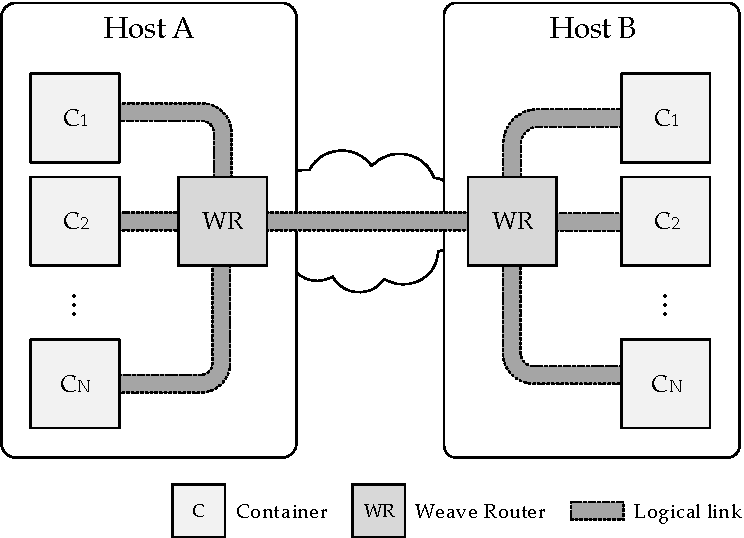
\includegraphics[width=0.7\textwidth]{figures/weave.pdf}
  \caption[An example of containers connected via \wnet\ overlay network]{A number of dispersed containers connected by a \wnet\ overlay network}\label{fig:weavescheme} 
\end{figure}

When the \weave\ software is started, a central component of \wnet , the \emph{\weave\ router} is launched (\cf\ \autoref{fig:weavescheme}). Similar to a hardware router, the \weave\ router is responsible for the forwarding and routing of data packets to their appropriate receivers. \weave\ routers can be seen as gateways through which all containers participating in a \weave\ network are connected. To facilitate routing on the data plane, a custom UDP encapsulation protocol, called \emph{sleeve}, was devised. A \weave\ router in itself is an containerized application running at all times, in the same way a daemon would. There is one of such router containers running on every host in a \weave -enabled infrastructure.

\todo[inline]{ÜBERARBEITEN}

The \weave\ router is a user space process. As such, a context switch is needed every time it is tasked to process a packet. This comes with a substantial performance overhead. Hence, as a faster alternative, the so-called \emph{fast datapath} mode was added. In this mode, packets are processed by the Linux kernel instead of by the \weave\ router. This way, the context switch into user space is omitted. \wnet\ leverages the Linux kernel's \emph{Open vSwitch datapath} module \cite{pfaff2015design} to achieve this behavior. Open vSwitch can be used to create a virtual, software-based network switch. That way, the kernel can be instructed to process packets in a certain way. For instance, the kernel can be commanded to add a VXLAN header to each packet, thereby achieving the same result as the \weave\ router, but faster. However, fast datapath mode can only be used when the underlying infrastructure allows it. The Internet is a particular example of a network where fast datapath communication is hard to achieve.


\subsection{Topology Management} 
\weave 's topology management is self-governing and self-healing. Peers continually exchange topology information and monitor the state of the network. Whenever peers lose connectivity, they continuously try to re-establish the connection until it is restored. All participating peers know the topology of the entire network. For this, \wnet\ employs a sophisticated discovery and topology management mechanism by which changes in the network topology are rapidly propagated within the network. The topology management protocol is based on a spanning-tree broadcast mechanism known from hardware switches. To further ensure that all peers have an up-to-date neighbor list at all times, \wnet\ additionally employs a custom neighbor gossiping protocol by which each peer sends update messages to a random subset of their neighbors. Updates of the network's topology are performed periodically as well as when certain events occur, such as when a node joins or leaves the network.

In order to add a new host to the overlay, the \weave\ software needs to be started on that host, referencing at least one other host in the network by its IP address. The information that a new host was added is then propagated to the other hosts in the overlay. After a short period, all hosts know that the new host was added and that a path to that host exists.

\subsection{Encryption} 
As mentioned earlier, a salient feature of \wnet\ is the ability to encrypt all traffic within the overlay network\footnote{Encryption applies end-to-end between \weave\ routers}. This is especially important for networks that span over insecure underlays, such as the Internet. To set up encryption, a shared secret (password) needs to be provided when the \weave\ router is launched. The shared secret must therefore be present on all participating hosts. From the password, salted, ephemeral session keys are generated which are then used to encrypt the network packets' payload. For each connection between any two peers, one unique session key exists.

The way encryption is applied differs depending on the forwarding mode used (sleeve or fast datapath). In fast datapath mode, a IPsec-based protocol is used, whereby each packet is wrapped in an encapsulated security payload (ESP). Because each packet in this mode is processed by the Linux kernel, encryption is applied by means of the standard Linux Kernel Crypto API which is thoroughly tested, and generally considered secure. For sleeve mode, a custom encryption algorithm based on TLS\footnote{``Transport Layer Security''} is used. As with fast datapath encryption, sleeve mode encryption utilizes shared, ephemeral session keys for each connection.

\begin{figure}[htpb]
  \centering
  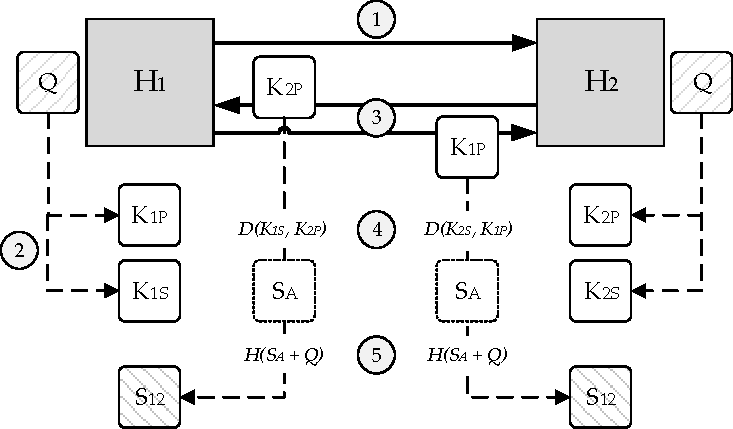
\includegraphics[width=0.6\textwidth]{figures/weave-encryption.pdf}
  \caption[\weave 's key exchange protocol]{\wnet 's key exchange protocol in sleeve mode}\label{fig:weaveencryption}
\end{figure} 
\autoref{fig:weaveencryption} depicts how these session keys are generated. In the image, two hosts ($H_1$, $H_2$) are to establish an encrypted connection. First, $H_1$ initiates the key exchange by sending a handshake message to $H_2$ \circled{1}. Then, both hosts generate their own, individual key pairs so that each host has a public key and a private key \circled{2}. The key pair for $H_1$ is $(K_{1P}, K_{1S})$ and the key pair for $H_2$ is $(K_{2P}, K_{2S})$. Once that is done, both hosts exchange their respective public keys, $K_{1P}$, and $K_{2P}$ \circled{3}. Using the peer's public key and their own private key, both hosts derive an auxiliary shared key, $S_A$, by means of Diffie--Hellman key exchange \cite{bresson2001provably}: $D(K_{1S},K_{2P})$ \circled{4}. Finally, the actual shared key can be generated. For this, both hosts append the password ($P$) to $S_A$ to provide authenticity. In order to bring the key to the desired length of 256 bit, the compounded key is additionally hashed via SHA256: $H(S_A, P)$ \circled{5}. The end result of this procedure is the final shared key, $S_{12}$, which is then used to encrypt the traffic between the two hosts.
%
%
%
%
%
%
%
%
%
%
%
%
%
%
%
%
%
%
%
%








